\documentclass[12pt]{article}
\usepackage[T5]{fontenc}
\usepackage[utf8]{inputenc}
\usepackage[english]{babel}
\usepackage{amsmath, amssymb}
\usepackage{graphicx}
\usepackage[colorlinks=true,
            linkcolor=blue,
            filecolor=magenta,
            urlcolor=cyan,
            citecolor=green,
            bookmarks=true,
            bookmarksopen=true]{hyperref}
\usepackage{enumitem}
\usepackage{geometry}
\geometry{margin=1in}
% \usepackage{listings}
\usepackage{minted}
\usepackage{xcolor}
\usepackage{caption}


\newminted[pythoncode]{python3}{linenos, style=vs_lm, framerule=0.5pt, frame=single, breaklines}

\title{Chapter 14 Report: \\ Classifying Images with CNNs}
\author{Quan Pham}
\date{\today}

\begin{document}

\maketitle
\tableofcontents
\newpage

\section{Abstract}
In this chapter, I studied convolutional neural networks (CNNs) and their application in image classification tasks. CNNs are designed to extract hierarchical features from images, which makes them highly effective for vision-related problems.

\section{Key Concepts}
\subsection{Sequential data}

Sequential data, also known as sequence data or sequences, is a type of data that its elements appear in a certain order, with interdependent relationships over time or position. The order of these elements is crucial, as it provide context and structural information that cannot be ignore during analysis. Changing the order can alter or even eliminate the meaning of the entire dataset. 

Sequential data can have different lengths, from short sequences to very long ones. These are some typical examples:
\textbf{Time series:} Daily stock price, sensor data (temperature, humidity), heart rate.
\textbf{Natural language:} Words in a sentence, sentences in a paragraph.
\textbf{Audio:} Voice waveforms, music sequences.
\textbf{Video:} Sequences of frames
\textbf{Biological sequence:} DNA sequences, protein sequences.

\subsection{Categories of sequence modeling}
If either the input or output is a sequence, the modeling task likely falls into one of these categories:
\begin{itemize}
    \item Many-to-one: The input data is a sequence, but the output is a fixed-size vector or scalar, not a sequence.
    \item One-to-many: The input data is in standard format and not a sequence, but the output is a sequence.
    \item Many-to-many: Both the input and output arrays are sequences. This category can be further divided based on whether the input and output are synchronized.
\end{itemize}

\subsection{Recurrent Neural Networks}
A recurrent neural network (RNN) is any network that contains a cycle within its network connections, meaning that the value of some unit is directly, or indirectly, dependent on its own earlier outputs as an input

Computing activation in an RNN is very similar to standard multilayer peerceptrons and other types of feedforward NNs. For the hidden layer, the net input (preactivation), is computed as follows:
\[\bm{z}_h^{(t)} = \bm{W}_{xh}\bm{x}^{(t)} + \bm{W}_{hh}\bm{h}^{(t-1)} + \bm{b}_h\]
Then, the activations of the hidden units at the time step, $t$, are calculated as follows:
\[\bm{h}^{(t)} = \sigma_h(\bm{z}_h^{(t)}) = \sigma_h(\bm{W}_{xh}\bm{x}^{(t)} + \bm{W}_{hh}\bm{h}^{(t-1)} + \bm{b}_h)\]
Once the activations of the hidden units at the current time step are computed, then the activations of the hidden units at the time step are computed, then the activations of the output units will be computed as follows:
\[\bm{o}^{(t)} = \sigma_o(\bm{W}_{ho}\bm{h}^{(t)} + \bm{b}_o)\]

\subsection{Challenges of learning long-range interactions}
Recurrent neural networks (RNNs) are theoretically capable of capturing dependencies across arbitrary sequence lengths. However, in practice, learning long-range interactions is challenging due to issues such as vanishing and exploding gradients during training. When backpropagating errors through many time steps, gradients can shrink exponentially (vanishing) or grow uncontrollably (exploding), making it difficult for the network to learn dependencies that span long intervals.

The vanishing gradient problem causes the network to "forget" information from earlier time steps, limiting its ability to model long-term dependencies. Conversely, exploding gradients can lead to unstable updates and numerical issues. 

% Various techniques have been proposed to address these challenges, including gradient clipping, careful initialization, and specialized architectures such as Long Short-Term Memory (LSTM) and Gated Recurrent Unit (GRU) networks, which introduce gating mechanisms to better preserve and control information flow over long sequences.

\section{Algorithms and Models Studied}
\subsection{Forward pass in convolution layer}
\begin{align*}
Z^{\text{conv}}[:,:,k] &= \sum_{c=1}^{C_{in}} W[:,:,c,k] * X[:,:,c] \\
Z[:,:,k] &= Z^{\text{conv}} + b[k] \\
A[:,:,k] &= \sigma(Z[:,:,k])
\end{align*}

\subsection{Adam optimization}
\textbf{Adam} (Adaptive Moment Estimation) is a widely used optimization algorithm in training neural networks. It combines the advantages of \textbf{AdaGrad} (adaptive learning rates for individual parameters) and \textbf{RMSprop} (using a moving average of squared gradients). Adam is effective due to its ability to adaptively adjust the learning rate for each parameter based on estimates of the first-order moments (mean) and second-order moments (variance) of the gradients.

\subsection*{Basic Steps:}
Given a learning rate $\alpha$, decay rates $\beta_1, \beta_2 \in [0, 1)$, and a small constant $\epsilon$ to prevent division by zero.
\begin{enumerate}
    \item Initialize moment vectors: $m_0 = \mathbf{0}$, $v_0 = \mathbf{0}$.
    \item For each iteration $t = 1, 2, \dots$:
    \begin{itemize}
        \item Compute the gradient $g_t$ of the loss function at time $t$:
        $$g_t = \nabla_\theta J(\theta_{t-1})$$
        \item Update biased first moment estimate (mean of gradients):
        $$m_t = \beta_1 m_{t-1} + (1 - \beta_1) g_t$$
        \item Update biased second moment estimate (mean of squared gradients):
        $$v_t = \beta_2 v_{t-1} + (1 - \beta_2) g_t^2$$
        \item Perform bias correction for the moments (to counteract initial values being zero):
        $$\hat{m}_t = \frac{m_t}{1 - \beta_1^t}$$
        $$\hat{v}_t = \frac{v_t}{1 - \beta_2^t}$$
        \item Update model parameters:
        $$\theta_t = \theta_{t-1} - \alpha \frac{\hat{m}_t}{\sqrt{\hat{v}_t} + \epsilon}$$
    \end{itemize}
\end{enumerate}

\subsection*{Advantages:}
\begin{itemize}
    \item \textbf{Efficiency:} Performs well in practice across various machine learning tasks.
    \item \textbf{Adaptive:} Adjusts the learning rate for each parameter, leading to faster convergence.
    \item \textbf{Ease of Use:} Does not require extensive hyperparameter tuning; default values often yield good results.
\end{itemize}

\subsection{Regularization}
\begin{itemize}
    \item L2 regularization (weight decay) and dropout help prevent overfitting.
    \item Dropout encourages robust feature learning.
\end{itemize}

\subsection{Other Techniques}
\begin{itemize}
    \item \textbf{Data augmentation}: enhances generalization.
    \item \textbf{Global average pooling}: reduces parameters.
\end{itemize}

\subsection{Example models in the book}
\begin{figure}[!h]
    \centering
    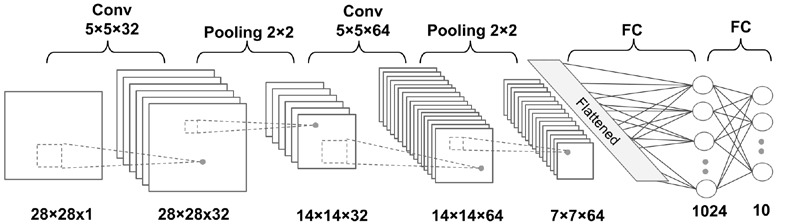
\includegraphics[width=0.9\textwidth]{../figures/deepCNN.jpg}
    \caption{A deep CNN}
\end{figure}


\section{Code Examples and Practical Exercises}
\subsection{Project one - predicting the sentiment of IMDb reviews}

\subsection{Project two - character-level language modeling with Pytorch}

\subsection{Practical Exploration with RNNs}

\section{Learnings and Challenges}
\subsection{Key Takeaways}

\subsection{Challenges Encountered}

\subsection{Opening Questions}

\section{Conclusion and Furture work}
Through this chapter, I have gained a comprehensive understanding of Convolutional Neural Networks (CNNs). I have learned how to utilize Python to implement CNNs for image classification tasks. Compared to neural networks consisting solely of fully connected layers, CNNs demonstrated significantly improved performance.

In subsequent chapters, I aim to delve into more advanced models, such as recurrent neural networks and transformers.

\nocite{mlbook2022}
\nocite{lecun1989handwritten}
\nocite{kingma2014adam}
\nocite{srivastava2014dropout}

% \newpage
% \section*{References}
% \addcontentsline{toc}{section}{References}
% \vspace{-0.5em}
% \begin{itemize}
%     \item LeCun et al. (1989), \textit{Handwritten Digit Recognition with a Back-Propagation Network}.
%     \item Krizhevsky et al. (2012), \textit{ImageNet Classification with Deep CNNs}.
%     \item Srivastava et al. (2014), \textit{Dropout: A Simple Way to Prevent Overfitting}.
%     \item Kingma and Ba (2014), \textit{Adam: A Method for Stochastic Optimization}.
% \end{itemize}

\bibliographystyle{plain}
\bibliography{references}

\end{document}
